\documentclass{ctexart}
\usepackage{array}

\usepackage{graphicx} %插入图片的宏包
\usepackage{float} %设置图片浮动位置的宏包
\usepackage{subfigure} %插入多图时用子图显示的宏包

   \title{UCAS-IHEP}                   %———总标题
   \author{yun}
%  
\begin{document}
   \maketitle                                  % —— 显示标题
\tableofcontents                               %—— 制作目录(目录是根据标题自动生成的)
   \section{China} %\label{1}                             %——一号子标题  China is in East Asia.
     \subsection{Shannxi}                      %——二号子标题  Beijing is the capital of China.
       \subsubsection{Xian}                    %——三号子标题
         \paragraph{XIDIAN UNIVERSITY}is a famous university.  %{}中的内容加粗显示
		   \subparagraph{School of telecommunication engineering} 
		   is in the best institute of XDU.
     \subsection{State Key Laboratory of ISN }
		 \paragraph{IHep} is the best university in communications industry. 
		 
		 \paragraph“天地玄黄,宇宙洪荒。日月盈昃,辰宿列张。”\footnote{出自《千字文》。}
		 
		 \begin{enumerate}
			\item An item.
			\begin{enumerate}
			\item A nested item.\label{itref}
			\item[*] A starred item.
			\end{enumerate}
			\item Reference(\ref{itref}).
			\end{enumerate}

	\section{排版}
		\subsection{对齐}
			% 居中对齐
			\begin{center}
			Centered text using a \verb|center| enviroment
			\end{center}
			% 左对齐
			\begin{flushleft}
			这是一个 \verb|flushleft| 环境
			\end{flushleft}
			% 右对齐
			\begin{flushright}
			这是一个 \verb|flushright| 环境
			\end{flushright}

			\centering
			Centered text paragraph.\par
			\raggedleft
			Left-aligned text paragraph.\par
			\raggedright
			Right-aligned text paragraph.\par
		\subsection{引用}
			yunxy once said:
			\begin{quote}
				“憋尿能行千里,拉稀寸步难行。”
			\end{quote}
			木兰诗
			\begin{quotation}
				万里赴戎机,关山度若飞。
				朔气传金柝,寒光照铁衣。
				将军百战死,壮士十年归。
				归来见天子,天子坐明堂。
				策勋十二转,赏赐百千强。……
			\end{quotation}
		\subsection{代码环境}
			\begin{verbatim}
				#include <iostream>

				int mian()
				{
					std::cout<<"hello world";
							 <<std::endl;

					return 0;
				}
			\end{verbatim}
			
			\begin{verbatim*}
				for(int i=0;i<=4;i++){
					cout<< i <<endl;
				}
			\end{verbatim*}
	\section{表格}
		\subsection{列格式}
			\begin{tabular}{l|c|r|p{6em}}
				\hline
				left&center&right
					&par box with fixed width\\
				L	&	C	&	R	&P	\\
				\hline
				
			\end{tabular}
			\par
			% 用@自定义文本
			\begin{tabular}{@{}r @{:}l| r @{}}
				\hline
				title \\
				\hline
				1 & 1 & one \\
				11 & 2 & eveleven \\
				\hline
			\end{tabular}
			\par
			\begin{tabular}{>{\itshape}r<{*}l}
				\hline
				italic & normal \\
				column & column \\
				\hline
			\end{tabular}
	\section{图片}
		\begin{figure}[H] %H为当前位置,!htb为忽略美学标准,htbp为浮动图形
			\centering%图片居中
			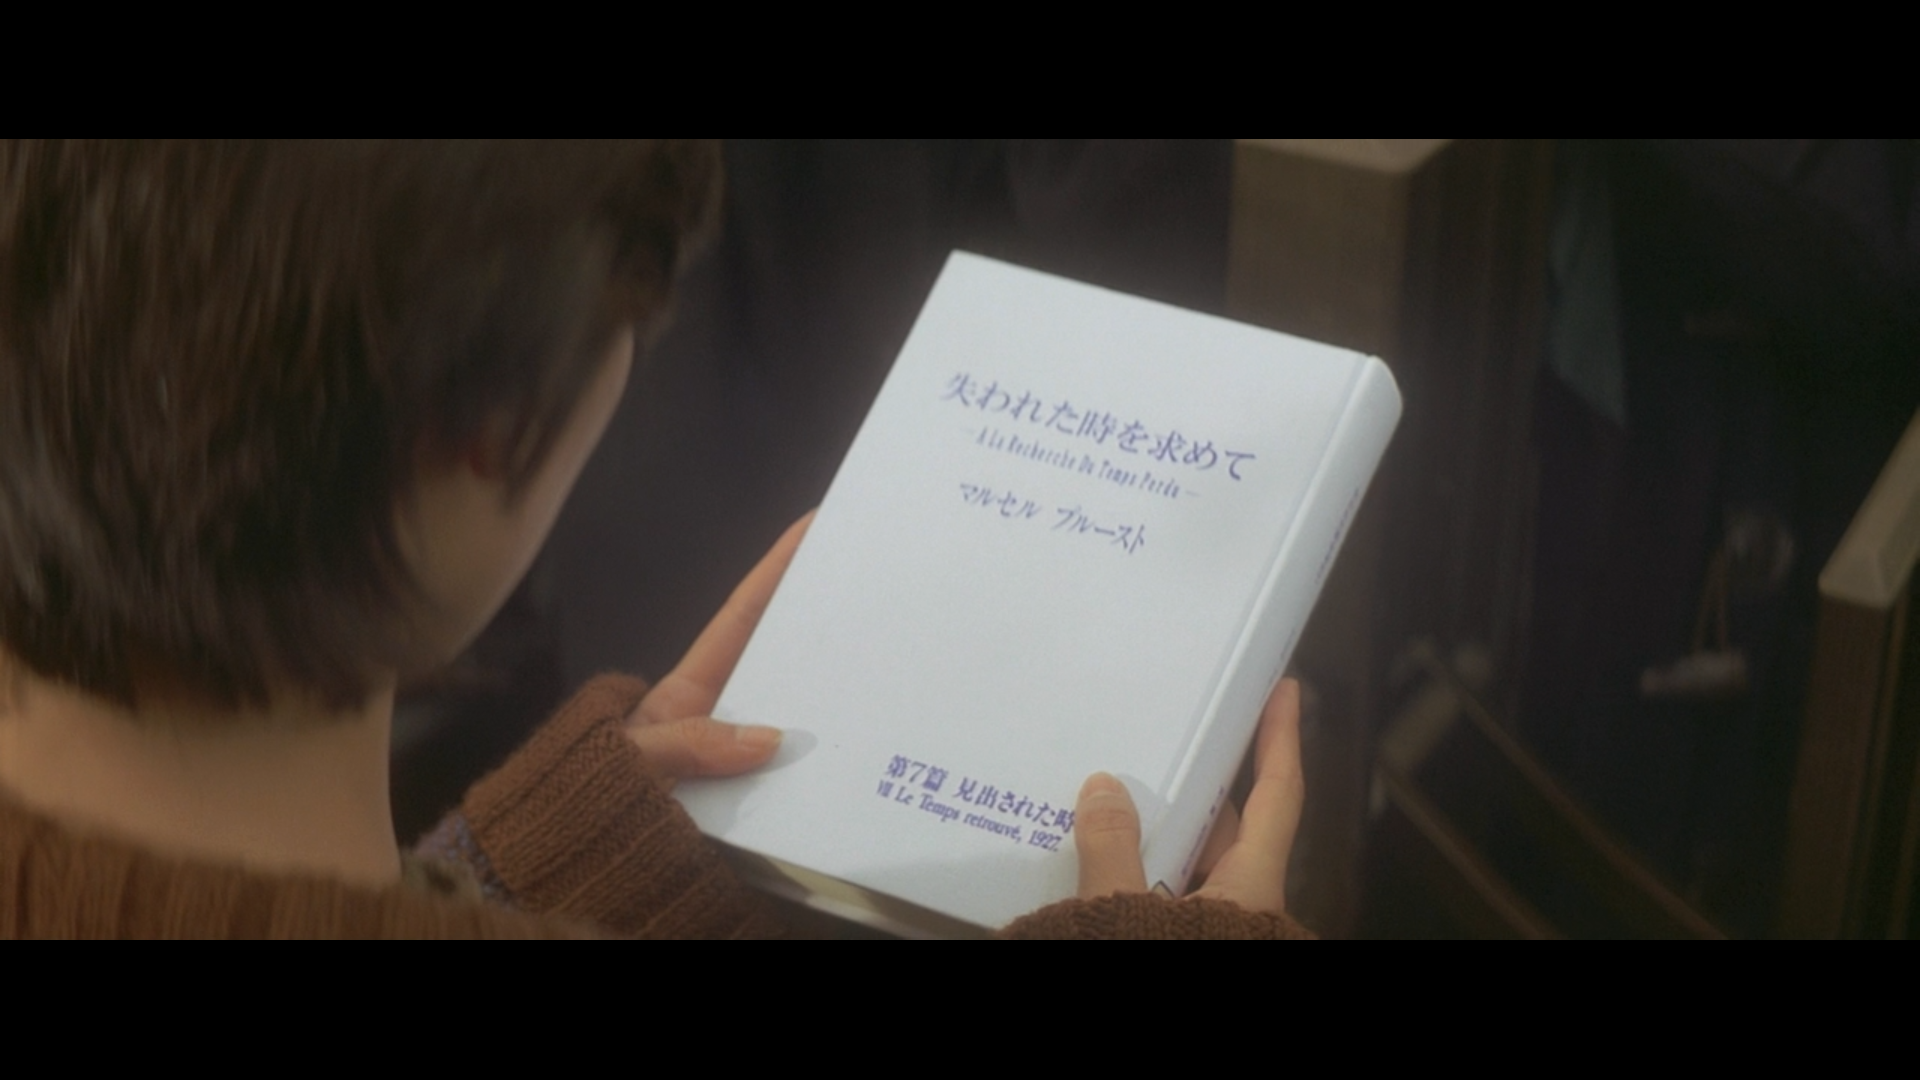
\includegraphics[width=0.7\textwidth]{1} %插入图片,[]中设置图片大小,{}中是图片文件名
			\caption{Main name2} %最终文档中希望显示的图片标题
			\label{Fig.main0} %用于文内引用的标签
		\end{figure}
		\begin{figure}[H]
			\centering  %图片全局居中
			\subfigure[图1]{
			\label{Fig.sub.1}
			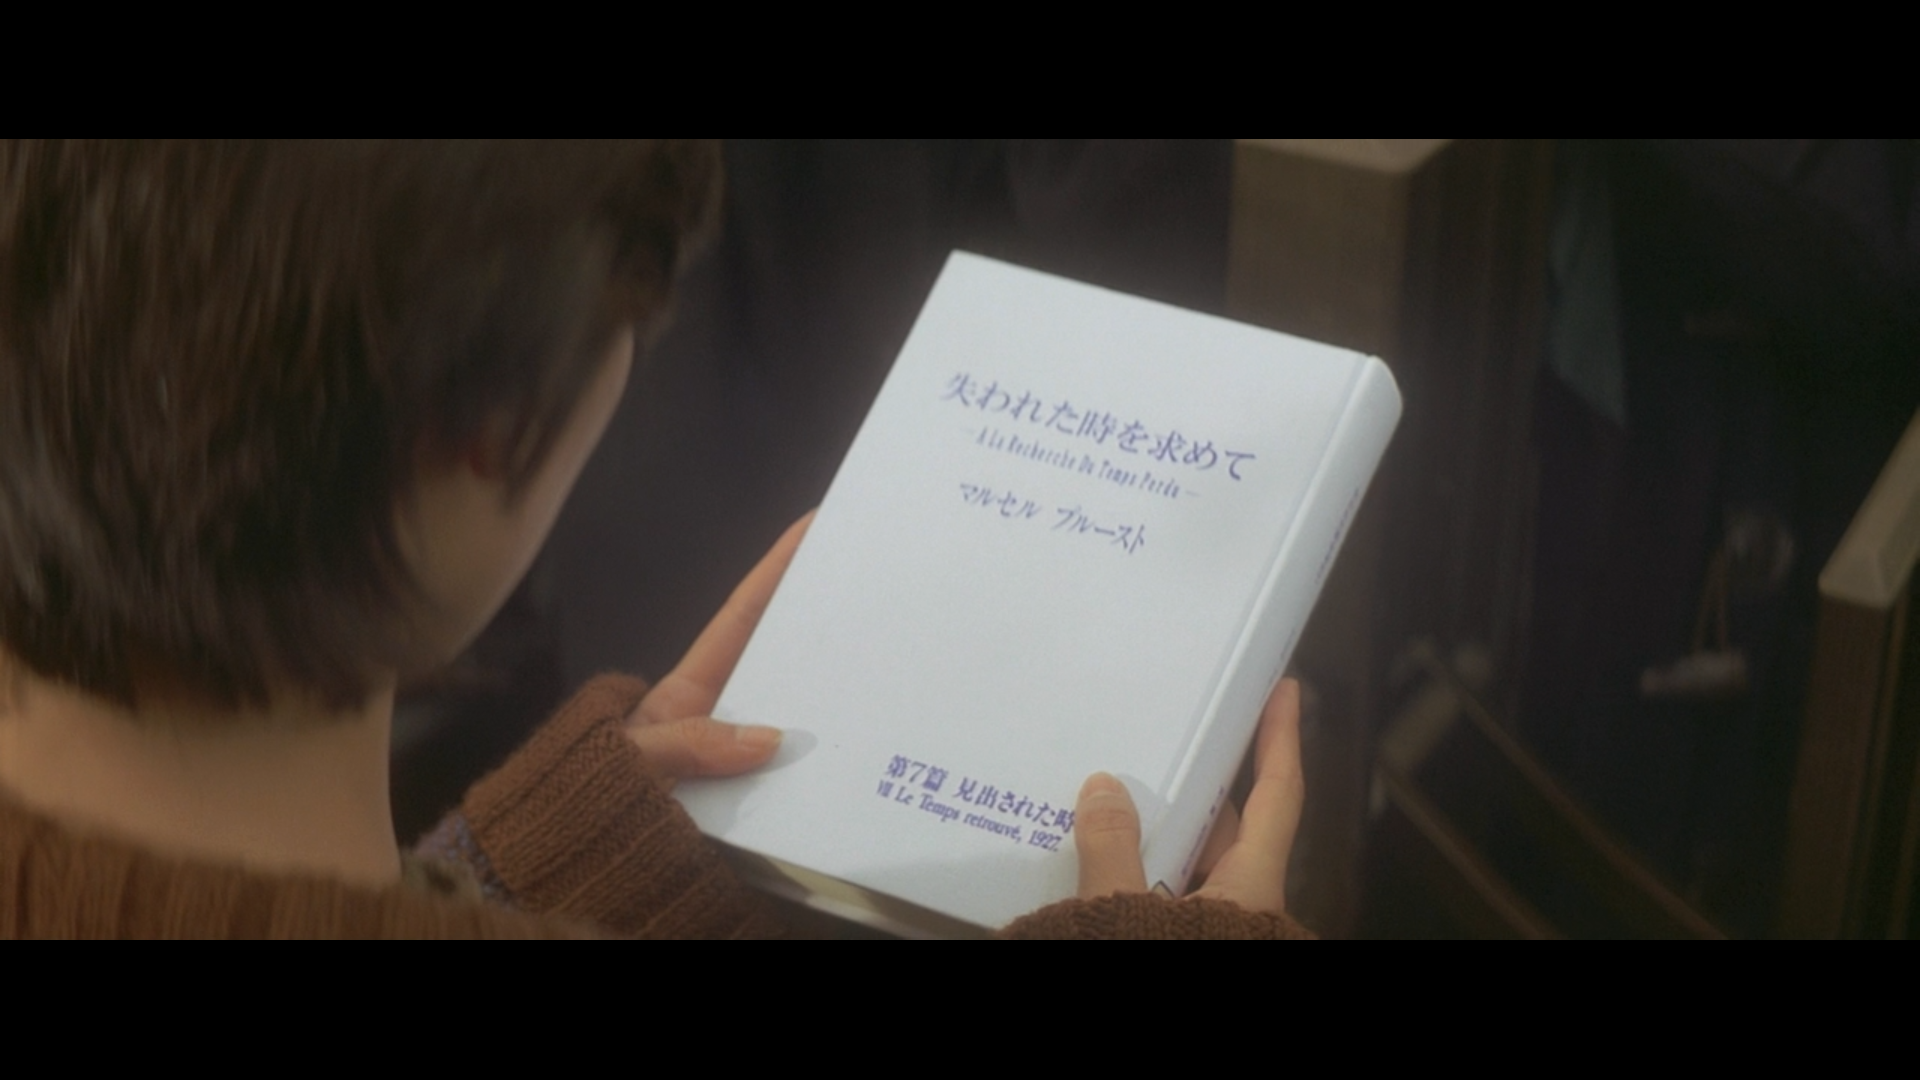
\includegraphics[width=0.45\textwidth]{1}}
			\subfigure[图2]{
			\label{Fig.sub.2}
			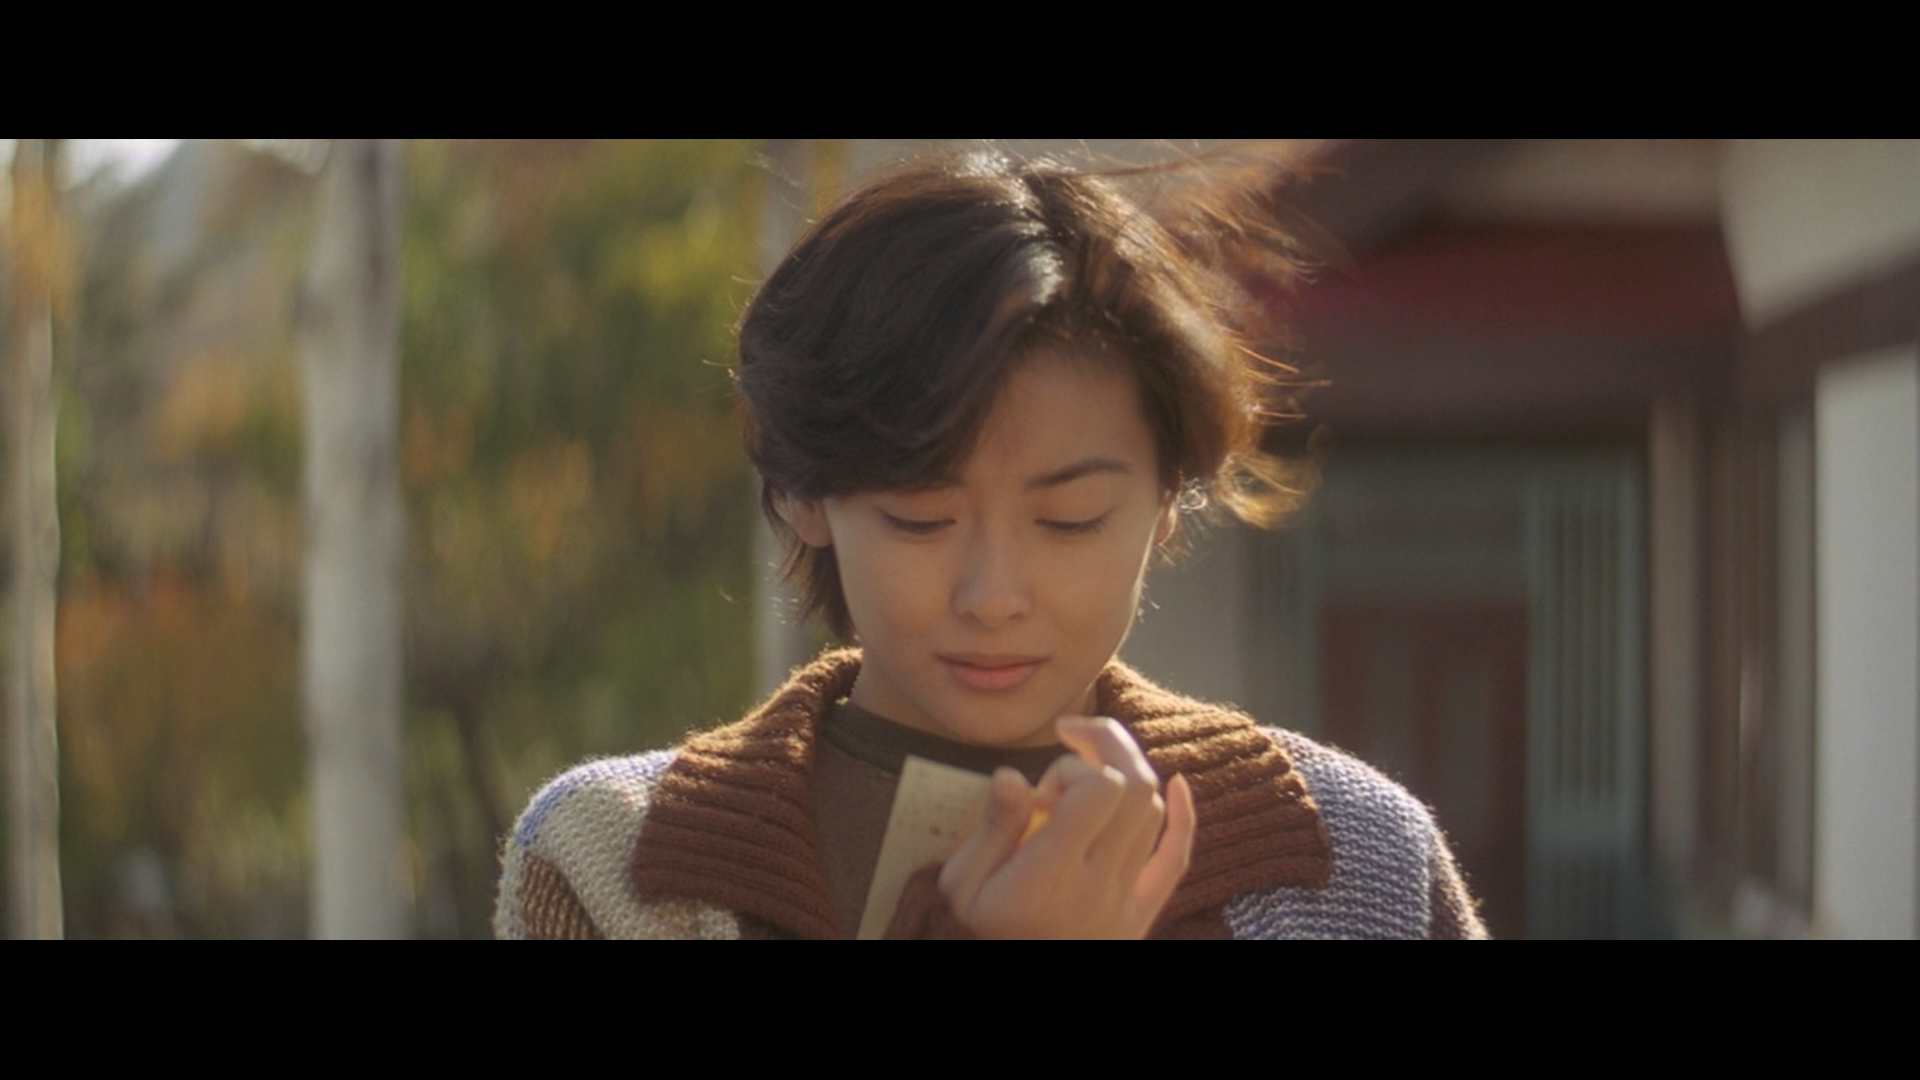
\includegraphics[width=0.45\textwidth]{2}}
			\caption{Main name}
			\label{Fig.main}
		\end{figure}

    \section{数学公式}
        $ \sin (x)/ x $
        In text :
        \[
        \lim_{n \to \infty} 
        \sum_{k=1}^n \frac{1}{k^2} 
        = \frac{\pi^2}{6}
        \]  \par
        $\frac{\pi^2}{6}$


% \appendix
% 	\section{append}
% 	\section{参考文献}
\end{document}